\chapter{Основные понятия и определения}
\selectlanguage{russian}

Изучение курса <<Защита информации>> необходимо начать с определения понятия \emph{<<информация>>}. В теоретической информатике \emph{информация} -- это любые сведения, или цифровые данные, или сообщения, или документы, или файлы, которые могут быть переданы \emph{получателю информации} от \emph{источника информации}. Можно считать, что информация передаётся по какому-либо каналу связи с помощью некоторого носителя, которым может быть, например, распечатка текста, диск или другое устройство хранения информации, система передачи сигналов по оптическим, проводным линиям или радиолиниям связи и~т.\,д.

\emph{Защита информации} -- это\footnote{Строго говоря, определение защиты информации даётся в официальном стандарте ГОСТ Р 50922-2006, <<Защита информации. Основные термины и определения>>~\cite{GOST-50922-2006}, согласно которому \emph{защита информации} -- это деятельность, направленная на предотвращение утечки защищаемой информации, несанкционированных и непреднамеренных воздействий на защищаемую информацию. Однако мы пользуемся определением, основанным на понятии <<безопасность информации>> из того же стандарта: \emph{безопасность информации} -- это состояние защищённости информации, при котором обеспечиваются ее \emph{конфиденциальность}, \emph{доступность} и \emph{целостность}.} обеспечение \emph{целостности}, \emph{конфиденциальности} и \emph{доступности} информации, передаваемой или хранимой в какой-либо форме. Информацию необходимо защищать от нарушения её целостности и конфиденциальности в результате вмешательства \emph{нелегального пользователя}. В российском стандарте ГОСТ Р 50.1.056-2005 приведены следующие определения~\cite{GOST-2005}:
\begin{itemize}
	\item \emph{целостность информации}\index{целостность} -- состояние информации, при котором отсутствует любое ее изменение, либо изменение осуществляется только преднамеренно субъектами, имеющими на него право;
	\item \emph{конфиденциальность}\index{конфиденциальность} -- состояние информации, при котором доступ к ней осуществляют только субъекты, имеющие на него право;
	\item \emph{доступность}\index{доступность} -- состояние информации, при котором субъекты, имеющие права доступа, могут реализовать их беспрепятственно.
\end{itemize}

Другой стандарт ГОСТ Р ИСО/МЭК 13335-1-2006~\cite{GOST-13335-1-2006} определяет \emph{информационную безопасность} как все аспекты, связанные с определением, достижением и поддержанием \emph{конфиденциальности}, \emph{целостности}, \emph{доступности}, \emph{неотказуемости}, \emph{подотчетности}, \emph{аутентичности} и \emph{достоверности} информации или средств ее обработки. То есть в дополнение к предыдущему определению на защиту информации в области информационных технологий возлагаются дополнительные задачи:
\begin{itemize}
	\item обеспечение \emph{неотказуемости} -- способность удостоверять имевшие место действие или событие так, чтобы эти события или действия не могли быть позже отвергнуты;
	\item обеспечение \emph{подотчетности} -- способность однозначно прослеживать действия любого логического объекта;
	\item обеспечение \emph{аутентичности} -- способность гарантировать, что субъект или ресурс идентичны заявленным;\footnote{Аутентичность применяется к таким субъектам, как пользователи, к процессам, системам и информации.}
	\item обеспечение \emph{достоверности} -- способность обеспечивать соответствие предусмотренному поведению и результатам;
\end{itemize}

Стандарт ГОСТ Р 50922-2006~\cite{GOST-50922-2006}, хотя и не вводит прямой классификации методов защиты информации, даёт следующие их определения.
\begin{itemize}
	\item \emph{Правовая защита информации}. Защита информации правовыми методами, включающая в себя разработку законодательных и нормативных правовых документов (актов), регулирующих отношения субъектов по защите информации, применение этих документов (актов), а также надзор и контроль за их исполнением.
	\item \emph{Техническая защита информации; ТЗИ}. Защита информации, заключающаяся в обеспечении некриптографическими методами безопасности информации (данных), подлежащей (подлежащих) защите в соответствии с действующим законодательством, с применением технических, программных и программно-технических средств.
	\item \emph{Криптографическая защита информации}. Защита информации с помощью ее криптографического преобразования.
	\item \emph{Физическая защита информации}. Защита информации путём применения организационных мероприятий и совокупности средств, создающих препятствия для проникновения или доступа неуполномоченных физических лиц к объекту защиты.
\end{itemize}

В рамках данного пособия в основном остановимся на криптографических методах защиты информации. Они помогают обеспечить \emph{конфиденциальность} и \emph{аутентичность}. В сочетании с правовыми методами защиты информации они помогают обеспечить \emph{неотказуемость} действий, а в сочетании с техническими -- \emph{целостность информации} и \emph{достоверность}.

При изучении криптографических методов защиты информации используются дополнительные определения. В целом науку о создании, анализе и использовании криптографических методов называют \emph{криптологией}. Её разделяют на \emph{криптографию}, посвящённую разработке и применению криптографических методов, и \emph{криптоанализ}, который занимается поиском уязвимостей в существующих методах. Данное разделение на криптографию и криптоанализ (и, соответственно, разделение на \emph{криптографов} и \emph{криптоаналитиков}) условно, так как создать хороший криптографический метод невозможно без умения анализировать его потенциальные уязвимости, а поиск уязвимостей в современных криптографических методах нельзя осуществить без знания методов их построения.

Попытка криптоаналитика нарушить свойство криптографической системы по обеспечению защиты информации (например, получить информацию вопреки свойству обеспечения конфиденциальности) называется \emph{криптографической атакой} (\emph{криптоатакой}). Если данная попытка оказалась успешной, и свойство было нарушено или может быть нарушено в ближайшем будущем, то такое событие называется \emph{взломом криптосистемы} или \emph{вскрытием криптосистемы}. Конкретный метод криптографической атаки также называется \emph{криптоанализом} (например, линейный криптоанализ, дифференциальный криптоанализ, и~т.~д.). Криптосистема называется \emph{криптостойкой}, если число стандартных операций для её взлома превышает возможности современных вычислительных средств в течение всего времени ценности информации (до 100 лет).

Для многих криптографических примитивов существует атака полным перебором\index{атака!полным перебором}, либо аналогичная, которая подразумевает, что если выполнить очень большое количество определённых операций (по одной на каждое значение из области определения одного из аргументов криптографического метода), то один из результатов укажет непосредственно на способ взлома системы (например, укажет на ключ для нарушения конфиденциальности, обеспечиваемой алгоритмом шифрования, или на допустимый прообраз для функции хэширования, приводящий к нарушению аутентичности и целостности). В этом случае под \emph{взломом криптосистемы} понимается построение алгоритма криптоатаки с количеством операций меньшим, чем планировалось при создании этой криптосистемы (часто, но не всегда, это равно именно количеству операций при атаке полным перебором\footnote{Например, сложность построения второго прообраза для хеш-функций на основе конструкции Меркла~---~Дамгарда составляет $2^n / \left|M\right|$ операций, тогда как полный перебор -- $2^n$. См. раздел~\ref{section-stribog}}). Взлом криптосистемы – это не обязательно, например, реально осуществленное извлечение информации, так как количество операций может быть вычислительно недостижимым как в настоящее время, так и в течение всего времени защиты. То есть могут существовать системы, которые формально взломаны, но пока ещё являются криптостойкими.

Далее рассмотрим модель передачи информации с отдельными криптографическими методами.

\section{Модель системы передачи с криптозащитой}
\selectlanguage{russian}

Простая модель системы передачи с криптозащитой представлена на рис.~\ref{pic:Encrypt}, где введены следующие обозначения:
\begin{itemize}
    \item $A$ -- источник информации;
    \item $B$ -- получатель информации, легальный пользователь;
    \item $X$ -- сообщение до шифрования или \emph{открытый текст}\index{открытый текст} (\langen{plaintext}); $\set{M}$ -- множество всех возможных открытых текстов (от слова Message), $X \in \set{M}$;
    \item $K_1$ -- ключ шифрования\index{ключ!шифрования} (\langen{encryption key}); $\set{K}_E$ -- множество всех возможных ключей шифрования, $K_1 \in \set{K}_E$;
    \item $Y$ -- зашифрованное сообщение (\emph{шифротекст}\index{шифротекст}, \langen{ciphertext, cyphertext} или \emph{шифрограмма}\index{шифрограмма}\footnote{Строго говоря, \emph{шифрограмма} -- это \emph{шифротекст} после его \emph{кодирования} для целей передачи по каналу связи.}); $\set{C}$ -- множество всех возможных шифротекстов, $Y \in \set{C}$;
    \item $K_2$ -- ключ расшифрования\index{ключ!расшифрования} (\langen{decryption key}); $\set{K}_D$  -- множество возможных ключей расшифрования, зависящее от множества $\set{K}_E$, $K_2 \in \set{K}_D$.
\end{itemize}

\begin{figure}[!thb]
	\centering
	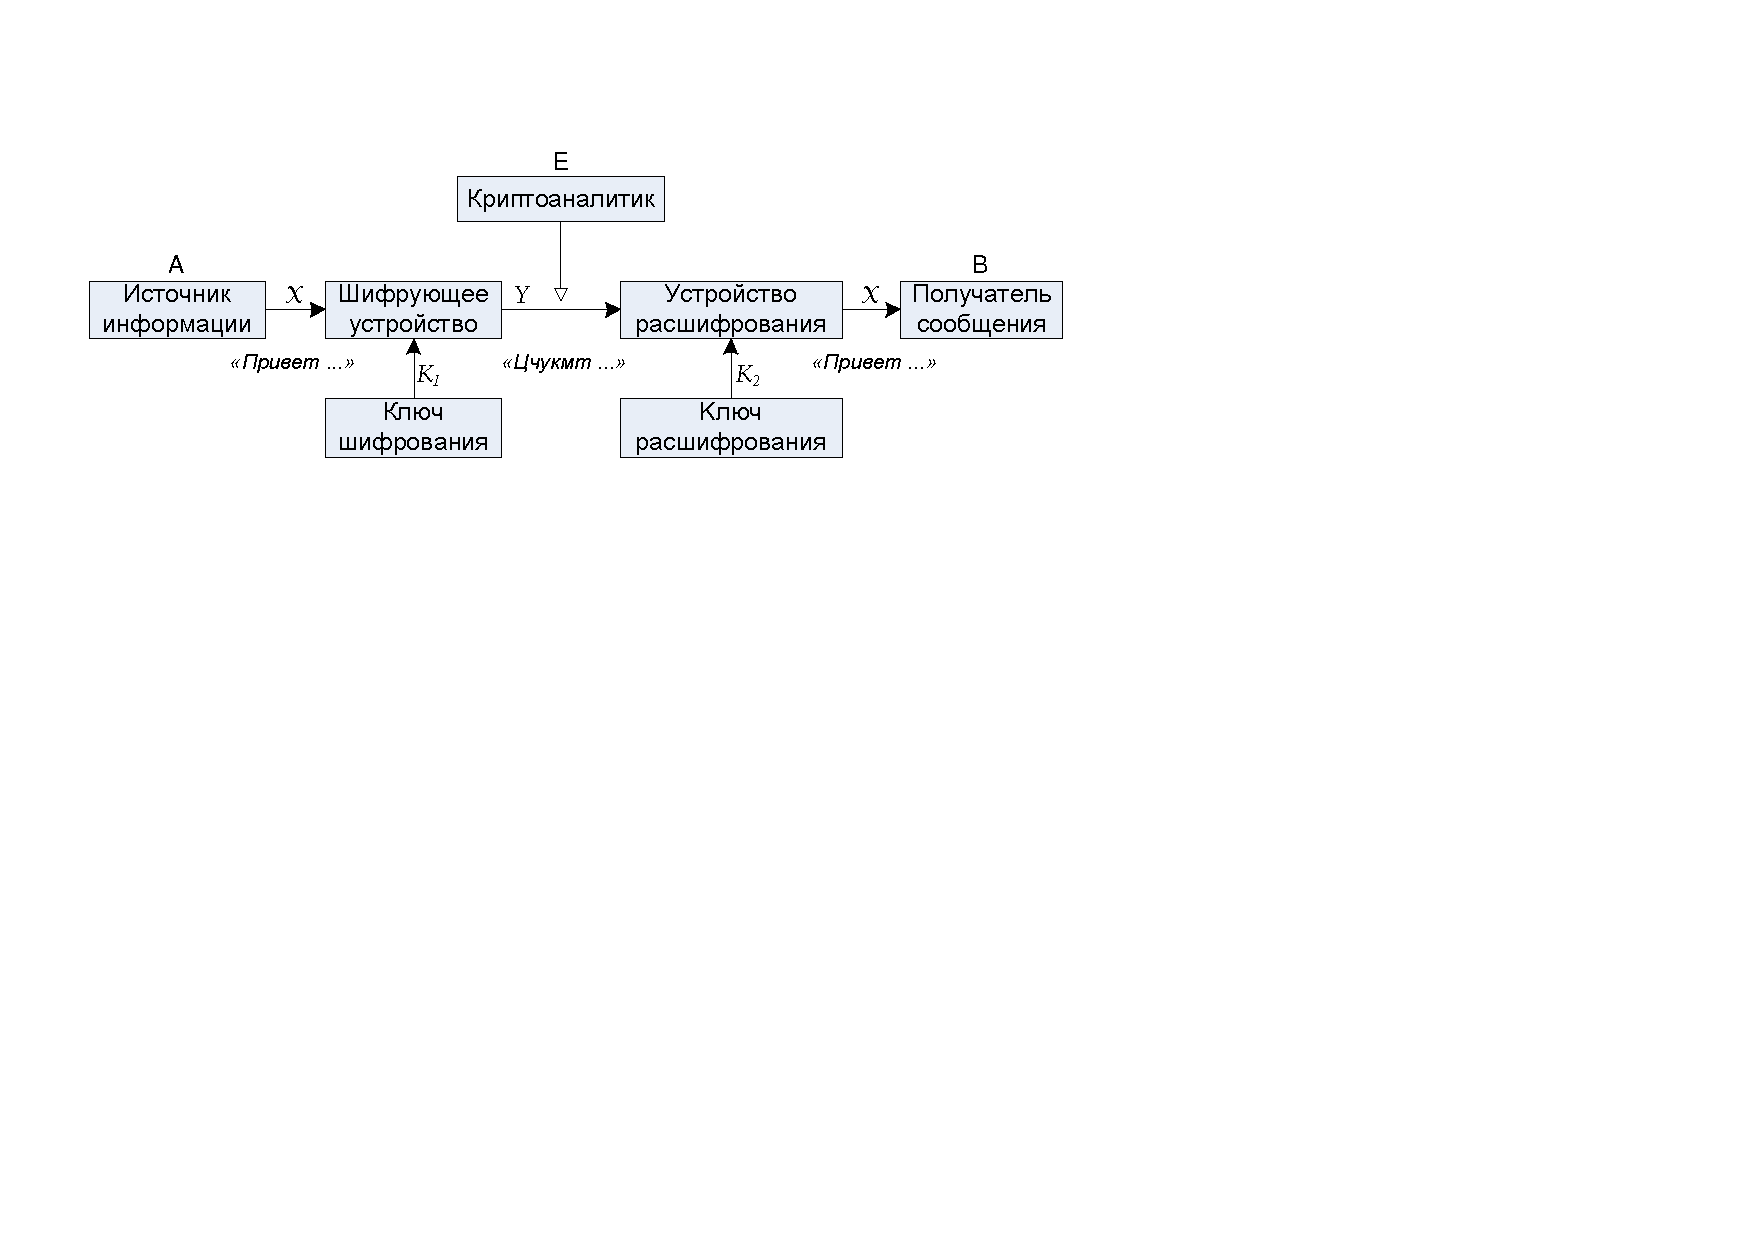
\includegraphics[width=1.0\textwidth]{pic/scheme-of-cipher}
	\caption{Передача информации с криптозащитой\label{pic:Encrypt}}
\end{figure}

\emph{Шифр}\index{шифр} -- это множество обратимых функций отображения $E_{K_1}$\index{функция!шифрования} множества открытых текстов $\set{M}$ на множество шифротекстов $\set{C}$, зависящих от выбранного ключа шифрования $K_1$ из множества $\set{K}_E$:
%обратимое отображение пары из элемента множества открытых текстов $\set{M}$ и элемента множества ключей шифрования $\set{K}_E$ в множество шифротекстов $\set{C}$:
\begin{equation}
    \label{eq:Encryption}
    Y = E_{K_1}(X), ~ X \in \set{M}, ~ K_1 \in \set{K}_E, ~ Y \in \set{C}.
\end{equation}
Можно сказать, что шифрование -- это обратимая функция двух аргументов: сообщения и ключа. Для каждого $K_1$ эта функция должна быть обратимой. Обратимость -- основное условие шифрования, по которому каждому зашифрованному сообщению $Y$ и ключу $K$ соответствует одно исходное сообщение $X$. Легальный пользователь $B$ (на приёмной стороне системы связи) получает сообщение $Y$ и осуществляет процедуру \emph{расшифрования}\index{расшифрование}.
Следует отличать шифрование от кодирования, так как кодирование -- это процесс сопоставления конкретным сообщениям строго определённой комбинации символов или сигналов, с целью повышения помехоустойчивости передаваемого сигнала.
Расшифрование -- это отображение множества шифротекстов $\set{C}$ в множество открытых текстов $\set{M}$ функцией $D_{K_2}$\index{функция!расшифрования}, зависящей от ключа расшифрования $K_2$ из множества $\set{K}_D$, являющейся обратной к функции $E_{K_1}$.
\begin{equation}
    \label{eq:Decryption}
    D_{K_2}(Y) = X, ~ Y \in \set{C}, ~ K_2 \in \set{K}_D, ~ X \in \set{M}.
\end{equation}

%Система передачи информации с криптозащитой называется \emph{криптосистемой}\index{криптосистема}.(?????)

%В общем случае функция шифрования сюръективна и псевдослучайна, отображая один открытый текст в разные шифротексты. Если функция шифрования биективна, на практике её инкапсулируют в другую функцию с целью добиться псевдослучайности шифрования одинаковых открытых текстов в разные шифротексты.

%Методы защиты информации зависят от возможных сценариев передачи. Рассмотрим несколько основных вариантов.
Рассмотрим возможные сценарии вмешательства криптоаналитика и организации защиты информации от его действий.
Пусть $A$ -- источник и $B$ -- получатель сообщений.

\begin{description}
    \item[Сценарий 1.] Пусть $E$ -- \emph{пассивный} криптоаналитик\index{криптоаналитик!пассивный}, который может подслушивать передачу, но не может вмешиваться в процесс передачи. Из пассивности криптоаналитика следует, что $Y = \widetilde{Y}$, и \emph{целостность} информации обеспечена.

Цель защиты --- \emph{обеспечение конфиденциальности}.

Средства защиты -- шифрование с помощью \emph{симметричных} или \emph{асимметричных } криптосистем.

Дополнительные задачи -- при большом числе пользователей должны быть решены задачи \emph{генерации и доставки секретных ключей} всем пользователям.

    \item[Сценарий 2.] Пусть $E$ -- \emph{активный} криптоаналитик\index{криптоаналитик!активный}, который может изменять, удалять и вставлять сообщения или их части.

    Цель защиты -- \emph{обеспечение конфиденциальности} и \emph{обеспечение целостности}.

Средства защиты -- шифрование и добавление \emph{имитовставки}\index{имитовставка} (message authentication code -- $\MAC$), позволяющее обнаружить нарушение целостности.

    \item[Сценарий 3.] Пусть $E$ -- активный криптоаналитик, который может изменять, удалять и вставлять сообщения или их части, дополнительно к этому легальные пользователи $A$ и $B$ не доверяют друг другу.

Цель защиты -- \emph{аутентификация} пользователей и документов.

Средства -- \emph{электронная подпись} и протокол идентификации (аутентификации) пользователей.
\end{description}

%%Возможно вмешательство нелегального пользователя $E$, называемого \emph{криптоаналитиком}.
%%
%%
%%Если $X = \widetilde{X}$, то вмешательство криптоаналитика $E$ не изменило передаваемое сообщение, и \emph{целостность} информации обеспечена. Если криптоаналитик не получил информацию, содержащуюся в сообщении, то обеспечена \emph{конфиденциальность}.
%%
%%Если в этой системе возможна двусторонняя передача, то есть от $A$ к $B$ и от $B$ к $A$, то говорят о взаимном обмене информацией между легальными пользователями.
%
%Секретность информации в современных шифрах обеспечивается секретным ключом, в то время как сам алгоритм криптосистемы является общеизвестным. Исторический опыт, например, система шифрования A5/1 в GSM, показывает, что секретность алгоритма шифрования \emph{ослабляет} криптостойкость шифра, а не увеличивает, из-за того, что система становится малоизученной.


\section[Классификация]{Классификация криптографических механизмов}

\subsection{Симметричные и асимметричные криптосистемы}
\selectlanguage{russian}

Криптографические системы и шифры можно разделить на две большие группы в зависимости от принципа использования ключей для шифрования и расшифрования.

Если для шифрования и расшифрования используется один и тот же ключ $K$, либо если получение ключа расшифрования $K_2$ из ключа шифрования $K_1$ является тривиальной операцией, то такая криптосистема называется \emph{симметричной}\index{криптосистема!симметричная}. В зависимости от объёма обработки данных за одну операцию шифрования симметричные шифры делятся на \emph{блочные}\index{шифр!блочный}, в которых за одну операцию шифрования происходит преобразование одного блока данных (32 бита, 64, 128 или больше), и \emph{потоковые}\index{шифр!потоковый}, в которых работают с каждым символом открытого текста по отдельности (например, с 1 битом или 1 байтом). Примеры блочных шифров рассмотрены в главе~\ref{chapter-block-ciphers}, а потоковых -- в главе~\ref{chapter-stream-ciphers}.

Шифрование блочным шифром подразумевает разделение открытого текста на блоки одинаковой длины. Блоки шифруются последовательно, причём результат шифрования следующего блока может зависеть от предыдущего. Это регулируется \emph{режимом сцепления блоков}. Примеры нескольких таких режимов рассмотрены в разделе~\ref{chapter-block-chaining}.

Если ключ расшифрования получить из ключа шифрования сложно (или невозможно), то такие криптосистемы называют криптосистемами \emph{с открытым ключом}\index{криптосистема!с открытым ключом} или \emph{асимметричными} криптосистемами\index{криптосистема!асимметричная}. Некоторые из них рассмотрены в главе~\ref{chapter-public-key}. Все используемые на сегодняшний день асимметричные криптосистемы работают с блоком данных открытого текста, представленным в виде числа длиной в несколько сотен или тысяч бит, поэтому классификация таких систем по объёму обрабатываемых за одну операцию данных не производится.

Алгоритм, который выполняет отображение аргумента произвольной длины в значение фиксированной длины, называется \emph{хэш-функцией}. Если для такой хэш-функции выполняются определённые свойства устойчивости к поиску коллизий, то это уже \emph{криптографическая хэш-функция}. Такие функции рассмотрены в главе~\ref{chapter-hash-functions}. Криптографические хэш-функции используются для проверки целостности сообщений. Для проверки с использованием общего секретного ключа отправителя и получателя используется механизм \emph{имитовставки}, рассмотренный в разделе~\ref{section-MAC}. Её аналогом в криптосистемах с открытым ключом является \emph{электронная подпись}, алгоритмы генерации и проверки которой рассмотрены в главе~\ref{chapter-public-key} вместе с алгоритмами асимметричного шифрования.

\subsection{Шифры замены и перестановки}

Шифры по способу преобразования открытого текста в шифртекст разделяются на шифры замены и шифры перестановки.

\subsubsection{Шифры замены}
\selectlanguage{russian}

В шифрах \textbf{замены} символы одного алфавита заменяются символами другого алфавита обратимым преобразованием. В последовательности открытого текста символы входного алфавита заменяются на символы выходного алфавита. Такие шифры применяются как в симметричных системах, так и в асимметричных криптосистемах. Если при преобразовании используются однозначные функции, то шифры замены называются однозначными шифрами замены. Если используются многозначные функции, то шифры называются многозначными шифрами замены (омофонами).

В \textbf{омофоне}\index{омофон} символам входного алфавита ставятся в соответствие непересекающиеся подмножества символов выходного алфавита. Количество символов в каждом подмножестве замены пропорционально частоте встречаемости символа открытого текста. Таким образом, омофон создает равномерное распределение символов шифротекста, и прямой частотный криптоанализ невозможен. При шифровании омофонами символ входного алфавита заменяется на случайно выбранный из подмножества замены.

Шифры бывают \textbf{моноалфавитные}, когда для шифрования используется одно отображение входного алфавита в выходной алфавит. Если алфавит на входе и выходе одинаков, и его размер (число символов) равен $D$, тогда количество всевозможных моноалфавитных шифров замены такого типа равно $D!$.

\textbf{Полиалфавитный} шифр задается множеством различных вариантов отображения входного алфавита на выходной алфавит. Шифры замены могут быть как потоковыми, так и блоковыми. Однозначный полиалфавитный потоковый шифр замены называется \textbf{шифром гаммирования}\index{шифр!гаммирования}. Символом алфавита может быть, например, 256-битовое слово, а размер алфавита -- $2^{256}$, соответственно.


\subsubsection{Шифры перестановки}
\selectlanguage{russian}

Шифры \textbf{перестановки} реализуются следующим образом. Берут открытый текст, например буквенный, и разделяют на блоки определённой длины $x_1, x_2, \dots, x_m$. Затем осуществляется перестановка позиций блока (вместе с символами). Перестановки могут быть однократные и многократные. Частный случай перестановки -- сдвиг. Приведём пример:
\begin{center}
    секрет $\xrightarrow{\text{сдвиг}}$ ретсек $\xrightarrow{\text{перестановка}}$ рскете.
\end{center}
Ключ такого шифра указывает изменение порядка номеров позиций блока при шифровании и расшифровании.

Существуют так называемые \textbf{маршрутные перестановки}. Используется какая-либо геометрическая фигура, например прямоугольник. Запись открытого текста ведётся по одному \emph{маршруту}, например по строкам, а считывание для шифрования осуществляется по другому маршруту, например по столбцам. Ключ шифра определяет эти маршруты.
В случае, когда рассматривается перестановка блока текста фиксированной длины, перестановку можно рассматривать как замену.

В полиалфавитных шифрах при шифровании открытый текст разбивается на блоки (последовательности) длины $n$, где $n$ -- \textbf{период}. Этот параметр выбирает \emph{криптограф} и держит его в секрете.

Поясним процедуру шифрования полиалфавитным шифром. Запишем шифруемое сообщение в матрицу по столбцам определённой длины. Пусть открытый текст таков: <<Игры различаются по содержанию, характерным особенностям, а также по тому, какое место они занимают в жизни детей>>. Зададим $n=4$ и запишем этот текст в матрицу размера $(4 \times 24)$:

\begin{center} \resizebox{\textwidth}{!}{ \begin{tabular}{|*{24}{c|}}
    \hline
    и&р&и&т&о&е&н&а&т&ы&о&н&я&а&п&м&к&е&о&а&а&ж&и&е \\
    г&а&ч&с&с&р&и&р&е&м&б&о&м&к&о&у&о&с&н&н&ю&и&д&й \\
    р&з&а&я&о&ж&ю&а&р&о&е&с&а&ж&т&к&е&т&и&и&т&з&е& \\
    ы&л&ю&п&д&а&х&к&н&с&н&т&т&е&о&а&м&о&з&м&в&н&т& \\
    \hline
\end{tabular} } \end{center}

Выбираем $4$ различных моноалфавитных шифра.

Первую строку

\begin{center} \resizebox{\textwidth}{!}{ \begin{tabular}{|*{24}{c|}}
    \hline
    и&р&и&т&о&е&н&а&т&ы&о&н&я&а&п&м&к&е&о&а&а&ж&и&е \\
    \hline
\end{tabular} } \end{center}

шифруем, используя первый шифр. Вторую строку

\begin{center} \resizebox{\textwidth}{!}{ \begin{tabular}{|*{24}{c|}}
    \hline
    г&а&ч&с&с&р&и&р&е&м&б&о&м&к&о&у&о&с&н&н&ю&и&д&й \\
    \hline
\end{tabular} } \end{center}

шифруем, используя второй шифр, и т.~д.

Выполняя расшифрование, легальный пользователь знает период. Он записывает принятую шифрограмму по строкам в матрицу с длиной строки равной периоду, к каждому столбцу применяет соответствующий ключ и расшифровывает сообщение, зная соответствующие шифры.

Шифры перестановки можно рассматривать как частный случай шифров замены, если отождествить один блок перестановки с одним символом большого алфавита.


\subsubsection{Композиционные шифры}
\selectlanguage{russian}

Почти все современные шифры являются \textbf{композиционными}~\cite{AlZKCh:2001}. В них применяются несколько различных методов шифрования к одному и тому же открытому тексту. Другое их название -- \textbf{составные шифры}. Впервые понятие составных шифров было введено в работе Клода Шеннона (\langen{Claude Elwood Shannon}).

В современных криптосистемах шифры замены и перестановок используются многократно, образуя составные (композиционные) шифры.



\subsection{Примеры современных криптографических примитивов}

Приведём примеры названий некоторых современных криптографических примитивов, из которых строят системы защиты информации.
\begin{itemize}
    \item DES\index{шифр!DES}, AES, ГОСТ 28147-89, Blowfish\index{шифр!Blowfish}, RC5\index{шифр!RC5}, RC6\index{шифр!RC6} -- блочные симметричные шифры, скорость обработки -- десятки мегабайт в секунду.
    \item A5/1, A5/2, A5/3\index{шифр!A5}, RC4\index{шифр!RC4} -- потоковые симметричные шифры с высокой скоростью. Семейство A5 применяется в мобильной связи GSM, RC4 -- в компьютерных сетях для SSL-соединения между браузером и веб-сервером.
    \item RSA\index{шифр!RSA} -- криптосистема с открытым ключом для шифрования.
    \item RSA\index{электронная подпись!RSA}, DSA\index{электронная подпись!DSA}, ГОСТ Р 34.10-2001\index{электронная подпись!ГОСТ Р 34.10-2001} -- криптосистемы с открытым ключом для электронной подписи.
    \item MD5\index{хэш-функция!MD5}, SHA-1\index{хэш-функция!SHA-1}, SHA-2\index{хэш-функция!SHA-2}, ГОСТ Р 34.11-94\index{хэш-функция!ГОСТ Р 34.11-94} -- криптографические хэш-функции.
\end{itemize}

\section{Методы криптоанализа и типы атак}
\selectlanguage{russian}

Нелегальный пользователь-криптоаналитик получает информацию путём дешифрования. Сложность этой процедуры определяется числом стандартных операций, которые надо выполнить для достижения цели. \emph{Двоичной сложностью}\index{сложность!двоичная} (или битовой сложностью) алгоритма называется количество двоичных операций, которые необходимо выполнить для его завершения.
% Наиболее сложным является дешифрование полиалфавитных шифров.

Рассмотрим основные сценарии работы криптоаналитика $E$. В первом сценарии криптоаналитик может осуществлять подслушивание и (или) перехват сообщений. Его вмешательство не нарушает целостности информации: $Y=\widetilde{Y}, где Y - целостность информации до вмешательства, \widetilde{Y} - целостность информации после вмешательства $. Эта роль криптоаналитика называется \emph{пассивной}. Так как он получает доступ к информации, то здесь нарушается конфиденциальность.

Во втором сценарии роль криптоаналитика \emph{активная}. Он может подслушивать, перехватывать сообщения и преобразовывать их по своему усмотрению: задерживать, искажать с помощью перестановок пакетов, устраивать обрыв связи, создавать новые сообщения и т.~п. В этом случае выполняется условие $Y \neq \widetilde{Y}$. Это значит, что одновременно нарушается целостность и конфиденциальность передаваемой информации.

Приведём примеры пассивных и активных атак:
\begin{itemize}
    \item Атака <<\emph{человек посередине}>>\index{атака!<<человек посередине>>} (\langen{man-in-the-middle}) подразумевает криптоаналитика, который разрывает канал связи, встраиваясь между $A$ и $B$, получает сообщения от $A$ и от $B$, а от себя отправляет новые, фальсифицированные сообщения. В результате $A$ и $B$ не замечают, что общаются с $E$, а не друг с другом.
    \item Атака \emph{воспроизведения}\index{атака!воспроизведения} (\langen{replay attack}) предполагает, что криптоаналитик может записывать и воспроизводить шифртексты, имитируя легального пользователя.
    \item Атака на \emph{различение} сообщений\index{атака!на различение} означает, что криптоаналитик, наблюдая одинаковые шифртексты, может извлечь информацию об идентичности исходных открытых текстов.
    \item Атака на \emph{расширение} сообщений\index{атака!на расширение} означает, что криптоаналитик может дополнить шифртекст осмысленной информацией без знания секретного ключа.
    \item \emph{Фальсификация} шифртекстов\index{атака!фальсификацией} криптоаналитиком без знания секретного ключа.
\end{itemize}

Часто для нахождения секретного ключа криптоатаки строят в предположениях о доступности дополнительной информации. Приведём примеры:
\begin{itemize}
    \item Атака на основе известного открытого текста\index{атака!с известным открытым текстом} (\langen{chosen plaintext attack, CPA}) предполагает, что криптоаналитик имеет возможность выбирать открытый текст и получать для него соответствующий шифртекст.
    \item Атака на основе известного шифртекста\index{атака!с известным шифртекстом} (\langen{chosen ciphertext attack, CCA}) предполагает возможность криптоаналитику выбирать шифртекст и получать для него соответствующий открытый текст.
\end{itemize}

Обязательным требованием к современным криптосистемам является устойчивость ко всем известным типам атак: пассивным, активным и с дополнительной информацией.


%Приведём примеры возможных вариантов работы активного криптоаналитика.
%\begin{itemize}
%\item Криптоаналитик имеет $m$ шифрованных сообщений $Y_{1},Y_{2},\ldots Y_{m}$ и пытается определить ключ или прочитать открытый текст $X_{1},X_{2},\ldots X_{m}.$
%\item Криптоаналитик имеет несколько пар открытого и шифрованного текстов
%
%$(Y_{1},X_{1}),(Y_{2}X_{2}),\ldots (Y_{m}X_{m})$ и пытается дешифровать остальной текст или определить алгоритм шифрования или определить ключ.
%\item
%\item
%\item
%\end{itemize}

Для защиты информации от активного криптоаналитика и обеспечения её целостности дополнительно к шифрованию сообщений применяют имитовставку\index{имитовставка}. Для неё используют обозначение $\MAC$ (\langen{message authentication code}). Как правило, $\MAC$ строится на основе хэш-функций, которые будут описаны далее.

Существуют ситуации, когда пользователи $A$ и $B$ не доверяют друг другу. Например, $A$ -- банк, $B$ -- получатель денег. $A$ утверждает, что деньги были переведены, $B$ - что перевода не было. Решение задачи аутентификации и неотрицаемости состоит в обеспечении \emph{электронной подписью}\index{электронная подпись} каждого из абонентов. Предварительно надо решить задачу о генерировании и распределении секретных ключей.

В общем случае системы защиты информации должны обеспечивать:
\begin{itemize}
    \item конфиденциальность\index{конфиденциальность} (защита от наблюдения),
    \item целостность\index{целостность} (защита от изменения),
    \item аутентификацию (защита от фальсификации пользователя и сообщений),
    \item доказательство авторства информации (доказательство авторства и защита от его отрицания)
\end{itemize}
как со стороны получателя, так и со стороны отправителя.

Важным критерием для выбора степени защиты является сравнение стоимости реализации взлома для получения информации и экономического эффекта от владения ей. Очевидно, что если стоимость взлома превышает ценность информации, взлом нецелесообразен.

%Сценарии защиты информации
%   Сценарий 1. A -- передающая сторона. B -- принимающая сторона. E -- пассивный
%криптоаналитик, который может подслушивать передачу, но не может вмешиваться
%в процесс передачи. Цель защиты: обеспечение конфиденциальности. Средства
%-- методы шифрования с секретным ключом (симметричные системы шифрования)
%и методы шифрования с открытым ключом (асимметричные системы шифрования).
%Сценарий 2. E -- активный криптоаналитик, который может изменять, удалять и вставлять
%сообщения или их части. Цель защиты -- обеспечение конфиденциальности (не
%всегда) и обеспечение целостности. Средства -- методы шифрования и добавление
%имитовставки\index{имитовставка} (Message Authentication Code -- $\MAC$).
%Сценарий 3. A и B не доверяют друг другу. Цель защиты -- аутентификация пользователя.
%Средства -- электронная подпись.


\section{Минимальные длины ключей}
\selectlanguage{russian}

Оценим минимальную битовую длину ключа для обеспечения криптостойкости, то есть защиты криптосистемы от атаки полным перебором всех возможных секретных ключей. Сделаем такие предположения:

\begin{itemize}
    \item одно ядро процессора выполняет $R = 10^7 \approx 2^{23}$ шифрований и расшифрований в секунду;
    \item вычислительная сеть состоит из $n = 10^3 \approx 2^{10}$ узлов;
    \item в каждом узле имеется $C = 16 = 2^4$ ядер процессора;
    \item нужно обеспечить защиту данных на $Y = 100$ лет, т.~е. на $S \approx 2^{32}$ с;
    \item выполняется закон Мура об удвоении вычислительной производительности на единицу стоимости каждые 2 года, то есть производительность вырастет в $M = 2^{Y/2} \approx 2^{50}$ раз.
\end{itemize}

Число переборов $N$ примерно равно
    \[ N \approx R \cdot n \cdot C \cdot S \cdot M, \]
    \[ N \approx 2^{23} \cdot 2^{10} \cdot 2^{4} \cdot 2^{32} \cdot 2^{50} = 2^{23+10+4+32+50} = 2^{119}. \]

Следовательно, минимально допустимая длина ключа для защиты от атаки перебором на 100 лет составляет порядка
    \[ \log_2 N \approx 119\text{ бит}. \]

Например, в 1997 году предыдущий американский стандарт шифрования DES с 56-битовым секретным ключом впервые был взломан перебором интернет-сетью из 78 000 частных компьютеров, производивших фоновые вычисления по проекту \textsc{DesChal}.

